\scanpage{64}
% block: numerical characters item 3
\handwritten{3}) The datum of the map
\[
\handwritten{\sigma\unsure{\mathrel{\begin{tikzpicture}[x=1cm,y=1cm,baseline=-.05cm]\draw[thin] (0,-.13)--(0,.15);\draw[thin] (0,0)--(.52,0).. controls (.57,0) and (.58,.03)..(.59,.08);\end{tikzpicture}}|\mapsto}}(Z_{\handwritten{\sigma}},\handwritten{\xi_\sigma})\ ,\ \handwritten{\xi_\sigma\in}\operatorname{Br}(Z_{\handwritten{\sigma}})
\]
considered in a).

% block: numerical characters item 4
4) The datum of the function
\[
\operatorname{rang}\ :\ \handwritten{\mathcal{M}\longrightarrow}\underline{Z}
\]
when $\handwritten{\mathcal{M}}$ is assumed\deleted{semi-}Tannakian.\deleted{\unsure{(i.e.}}

% block: effective part
It will be noted that the datum of 1),2) is equivalent to the datum of the commutative ring $K=K(\handwritten{\mathcal{M}})$, with its ``effective part
\[
\begin{aligned}
K^{\mathrm{eff}}&=\text{subgroup of }K(\handwritten{\mathcal{M}})\text{ generated by the}\\
&\qquad c\handwritten{\ell}(M),\ M\handwritten{\in}\operatorname{Ob}\quad,\\
&=\underline{N}^{(\handwritten{\Sigma})}
\end{aligned}
\]
(NB $\handwritten{\Sigma}$ is recovered from \deleted{\unsure{these}}\inserted{\handwritten{the}} datum\inserted{\handwritten{$K^{\mathrm{eff}}\subset K$\begin{tikzpicture}[x=1cm,y=1cm,baseline=-.1cm]\draw[thin] (0,.12).. controls (.05,-.08) and (-.1,-.1)..(-.5,-.12)--(-1.6,-.12).. controls (-1.85,-.12) and (-1.95,-.28)..(-1.93,-.5);\end{tikzpicture}}} as the set of minimal nonzero eleme\unsure{nts} of $K^{\mathrm{eff}}$). The datum of 3) then makes it possible to find, as made explicit in a), the functorial variance of the ring $K(\handwritten{\mathcal{M}}_{k'})$ with respect to $k'$. Finally the datum of 4) makes it possible in principle to recover the characteristic polynomials (in particular, the trace and the determinant) of an endomorphism of an object \deleted{of}(semi-simple ?) $M$ of $E$, in \unsure{\deleted{e}t|\deleted{o}t|\deleted{t}e}erms of reduced characteristic polynomials (resp. reduced trace, reduced norm) in the Azumaya algebras\inserted{$\operatorname{End}(M_i)$,\begin{tikzpicture}[x=1cm,y=1cm,baseline=-.1cm]\draw[thin] (0,.12).. controls (.05,-.08) and (-.1,-.1)..(-.5,-.12)--(-1.6,-.12).. controls (-1.85,-.12) and (-1.95,-.28)..(-1.93,-.5);\end{tikzpicture}} corresponding to the isotypic components $M_i$ of $M$. For $M$ isotypic of rank $n$, we shall indeed have, if $K=\operatorname{End}(M)$ has as centre $Z$ of rank $r$ over $k$, hence $n=n'\unsure{\deleted{d}r|\deleted{r}d}$, and $K$ of rank $d^2$ over $Z$, with $d\handwritten{\mid}n'$ (NB $M$ of rank $n'$ over $Z$):
\diagram{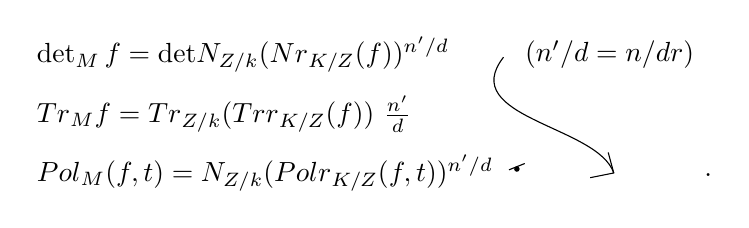
\begin{tikzpicture}[x=1cm,y=1cm]
\node[anchor=west] at (0,0) {$\det_M f=\deleted{\det}N_{Z/k}(\operatorname{Nr}_{K/Z}(f))^{n'/d}$};
\node[anchor=west] at (0,-.75) {$\operatorname{Tr}_M f=\operatorname{Tr}_{Z/k}(\operatorname{Trr}_{K/Z}(f))\ \frac{n'}{d}$};
\node[anchor=west] at (0,-1.5) {$\operatorname{Pol}_M(f,t)=N_{Z/k}(\operatorname{Polr}_{K/Z}(f,t))^{n'/d}$};
\node[anchor=west] at (6.2,0) {$\inserted{(n'/d=n/dr)}$};
\draw[thin] (6.05,-.03).. controls (5.45,-.8) and (7.25,-.9)..(7.45,-1.5);
\draw[thin] (7.15,-1.56)--(7.45,-1.5)--(7.38,-1.24);
\draw[thin] (6.12,-1.46)--(6.32,-1.38);\fill (6.22,-1.45) circle (.035);
\node at (8.65,-1.52) {$.$};
\end{tikzpicture}}
\margin{\handwritten{\unsure{Point out} that knowledge of the numerical characters of $\mathcal{M}$ implies that of the numerical characters of $\mathcal{M}_{k'}$ for \unsure{any} extension $k'$ of $k$, (``functorial in $k'$'')}}

% block: warning about reconstruction
One should be aware that knowledge of the numerical characters of the Tannakian category $\handwritten{\mathcal{M}}$ does not in general make it possible to reconstruct it up to equivalence, even if $k$ is an algebraically closed field of characteristic 0 (so that the datum of 3) becomes empty) and $\handwritten{\mathcal{M}}$ semi-simple
% archive sheet number: 63
